% Chapter 4: Design and Implementation

\chapter{Diseño e implementación} % Main chapter title

\label{Chapter4} % Reference

%----------------------------------------------------------------------------------------

\section{Arquitectura de seguridad}

%----------------------------------------------------------------------------------------

\section{Arquitectura del software}

Para explicar la arquitectura software de la aplicación, esta sección va a estar dividida en varios
prototipos que se han desarrollado:

\subsection{Shatter 0.1}

El primer prototipo de la aplicación se desarrolló enteramente en Java, usando para ello el entorno
de desarrollo Eclipse. Esta primera versión buscaba poder dividir un fichero en varios fragmentos
de un tamaño dado, y luego poder recomponerlo. Para ello se implementaron algunas clases:

\begin{itemize}
  \item \keyword{Slice} -- Un Slice es uno de los fragmentos en los que un
  fichero original se ha dividido. Está formado por una cabecera (Header) y un
  array de bytes en el que se almacena el contenido del segmento del fichero.
  (Figura~\ref{fig:Slice_Header_1})

  \item \keyword{Header} -- En esta clase se almacenan los metadatos de los
  Slices. Se guardan datos como un contador, el número total de Slices
  para un fichero, un ID para la sesión\footnote{En esta primera iteración de la
  aplicación, el ID para identificar la sesión era un resumen Hash del fichero.}
  y el tamaño original del fichero. (Figura~\ref{fig:Slice_Header_1})

  \item \keyword{Slicer} -- Esta clase es la \emph{fábrica} de Slices. Recibe
  un fichero, un tamaño de bloque y un ID para identificar la sesión. Lee del
  fichero bloques del tamaño indicado hasta alcanzar el EOF y genera un Slice
  para cada uno de ellos, con una cabecera distinta. (Figura~\ref{fig:Assembler})

  \item \keyword{Composer} -- Si el anterior recibía un fichero y generaba Slices,
  éste recibe Slices y devuelve un fichero compuesto. Lee uno a uno los Slices
  que recibe, prestando especial atención a sus cabeceras y si detecta que
  alguno falta genera un log de errores. (Figura~\ref{fig:Assembler})
\end{itemize}

\begin{figure}[ht]
  \centering
  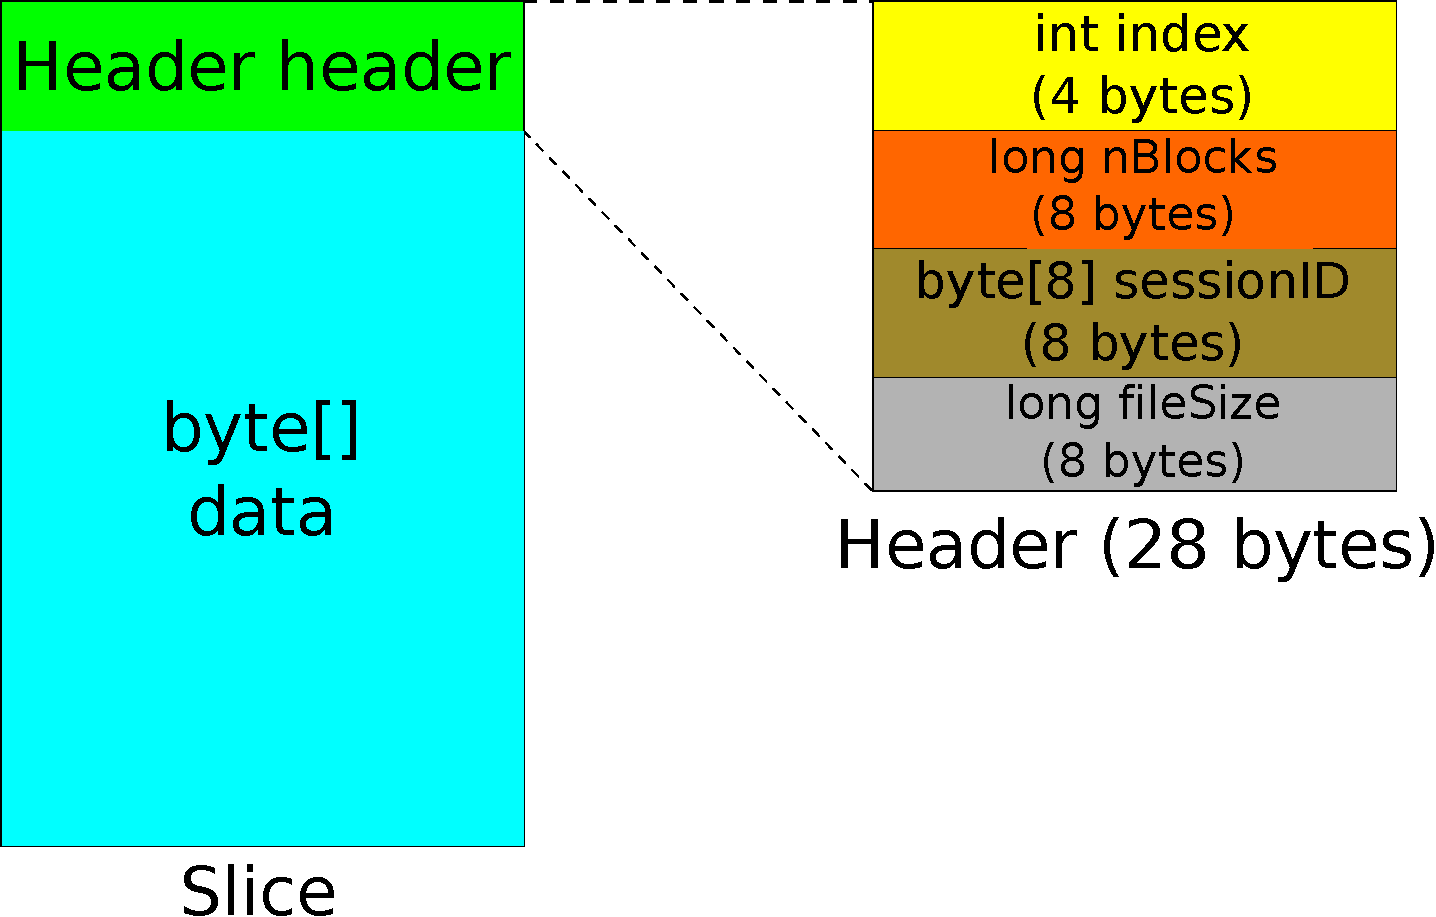
\includegraphics[scale=0.4]{Figures/Slice_Header_1}
  \decoRule
  \caption[Slice - Header (Versión 1)]{Esquema general de las clases Slice y Header (Versión 1)}
  \label{fig:Slice_Header_1}
\end{figure}

\begin{figure}[ht]
  \centering
  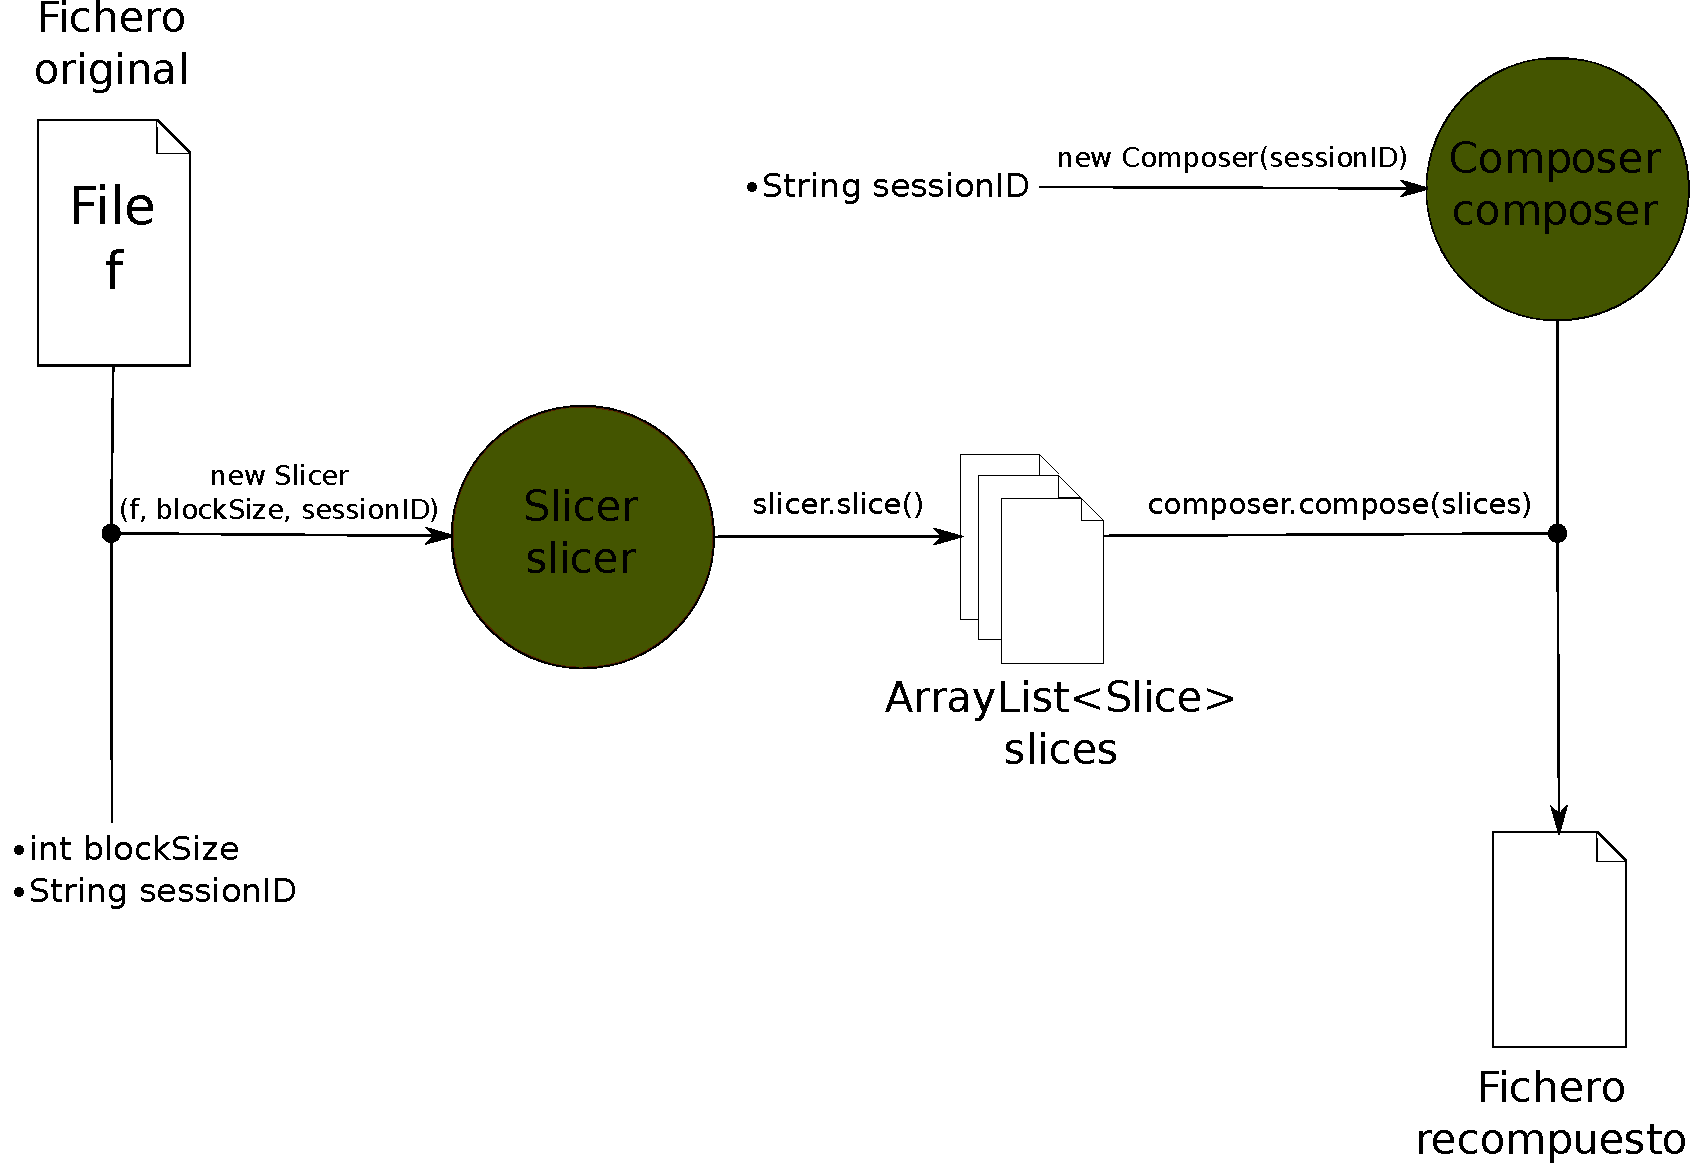
\includegraphics[scale=0.5]{Figures/Assembler}
  \decoRule
  \caption[Slicer - Composer]{Esquema general del Slicer y el Composer}
  \label{fig:Assembler}
\end{figure}

Al tratarse de un prototipo bastante sencillo, no dió muchos problemas, se
alcanzaron fácilmente los objetivos buscados.

\subsection{Shatter 0.5}

En esta segunda versión, el objetivo era proporcionar confidencialidad a las
Slices. Para llevarlo a cabo se implementaron las siguientes clases:

\begin{itemize}
  \item \keyword{EncFile} -- Viene a ser una Slice cifrada. A parte de los datos
  encriptados de la Slice, también incluye una cabecera (EncFileHeader) con
  algunos datos importantes y una pseudocabecera (FalseHeader) con datos menores.
  (Figura~\ref{fig:EncFile_Header_1})

  \item \keyword{EncFileHeader} -- Como decía antes, esta cabecera se usa para
  almacenar algunos metadatos importantes como, en este caso, el vector de
  inicialización (IV) que se ha usado para cifrar la Slice.
  (Figura~\ref{fig:EncFile_Header_1})

  \item \keyword{KeyFile} -- Esta clase se utiliza para almacenar la clave
  simétrica que se ha utilizado para crear los EncFiles.

  \item \keyword{AESLibrary} -- Básicamente, una clase que se encarga de
  generar de manera aleatoria y segura claves simétricas y vectores de
  inicialización.

  \item \keyword{SymmetricCipher} -- Esta es la clase que se encarga de hacer
  la parte más importante en cuanto a la confidencialidad. Una vez que ha sido
  inicializado con una clave simétrica, genera textos cifrados a partir de
  texto plano y un IV. Igualmente, puede llevar a cabo el proceso inverso.

  \item \keyword{Encryptor} -- La \emph{fábrica} de EncFiles. Genera de manera
  aleatoria y segura (Utilizando una de las clases mencionadas anteriormente)
  una clave simétrica para un algoritmo establecido y, con ella, inicializa una
  instancia de un SymmetricCipher. A continuación se le pasa un array de Slices
  del cual genera un array de EncFiles, que es el que retorna.
  (Figura~\ref{fig:Encryptor})

  \item \keyword{Decryptor} -- La contraparte del Encryptor. Realiza el proceso
  inverso y devuelve un array de Slices a partir de uno de EncFiles.
  (Figura~\ref{fig:Decryptor})
\end{itemize}

\begin{figure}[ht]
  \centering
  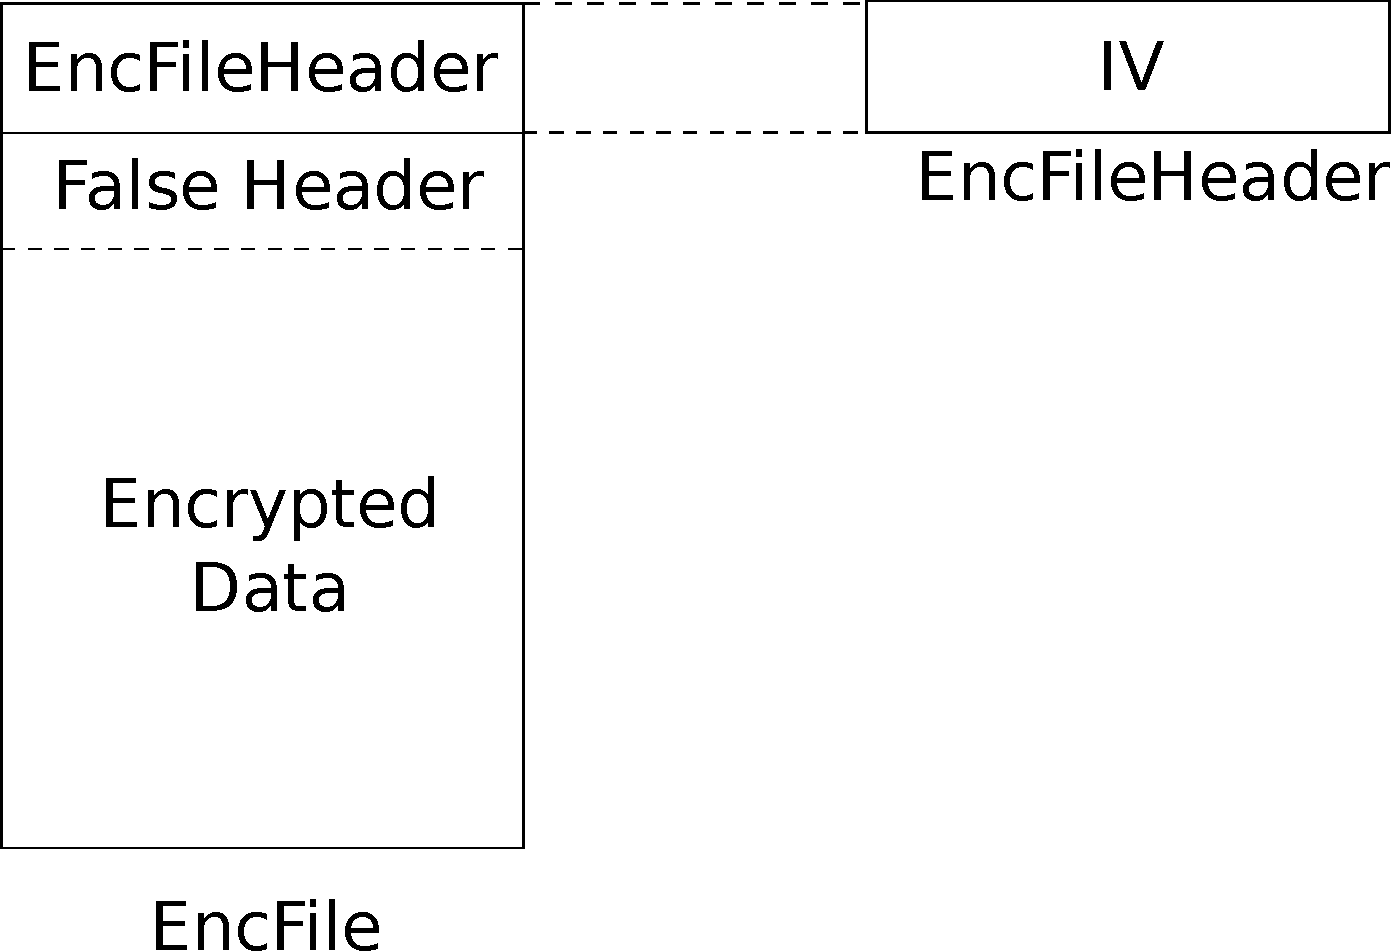
\includegraphics[scale=0.4]{Figures/EncFile_Header_1}
  \decoRule
  \caption[EncFile - EncFileHeader (Versión 1)]{Esquema general de las clases EncFile y EncFileHeader (Versión 1)}
  \label{fig:EncFile_Header_1}
\end{figure}

\begin{figure}[ht]
  \centering
  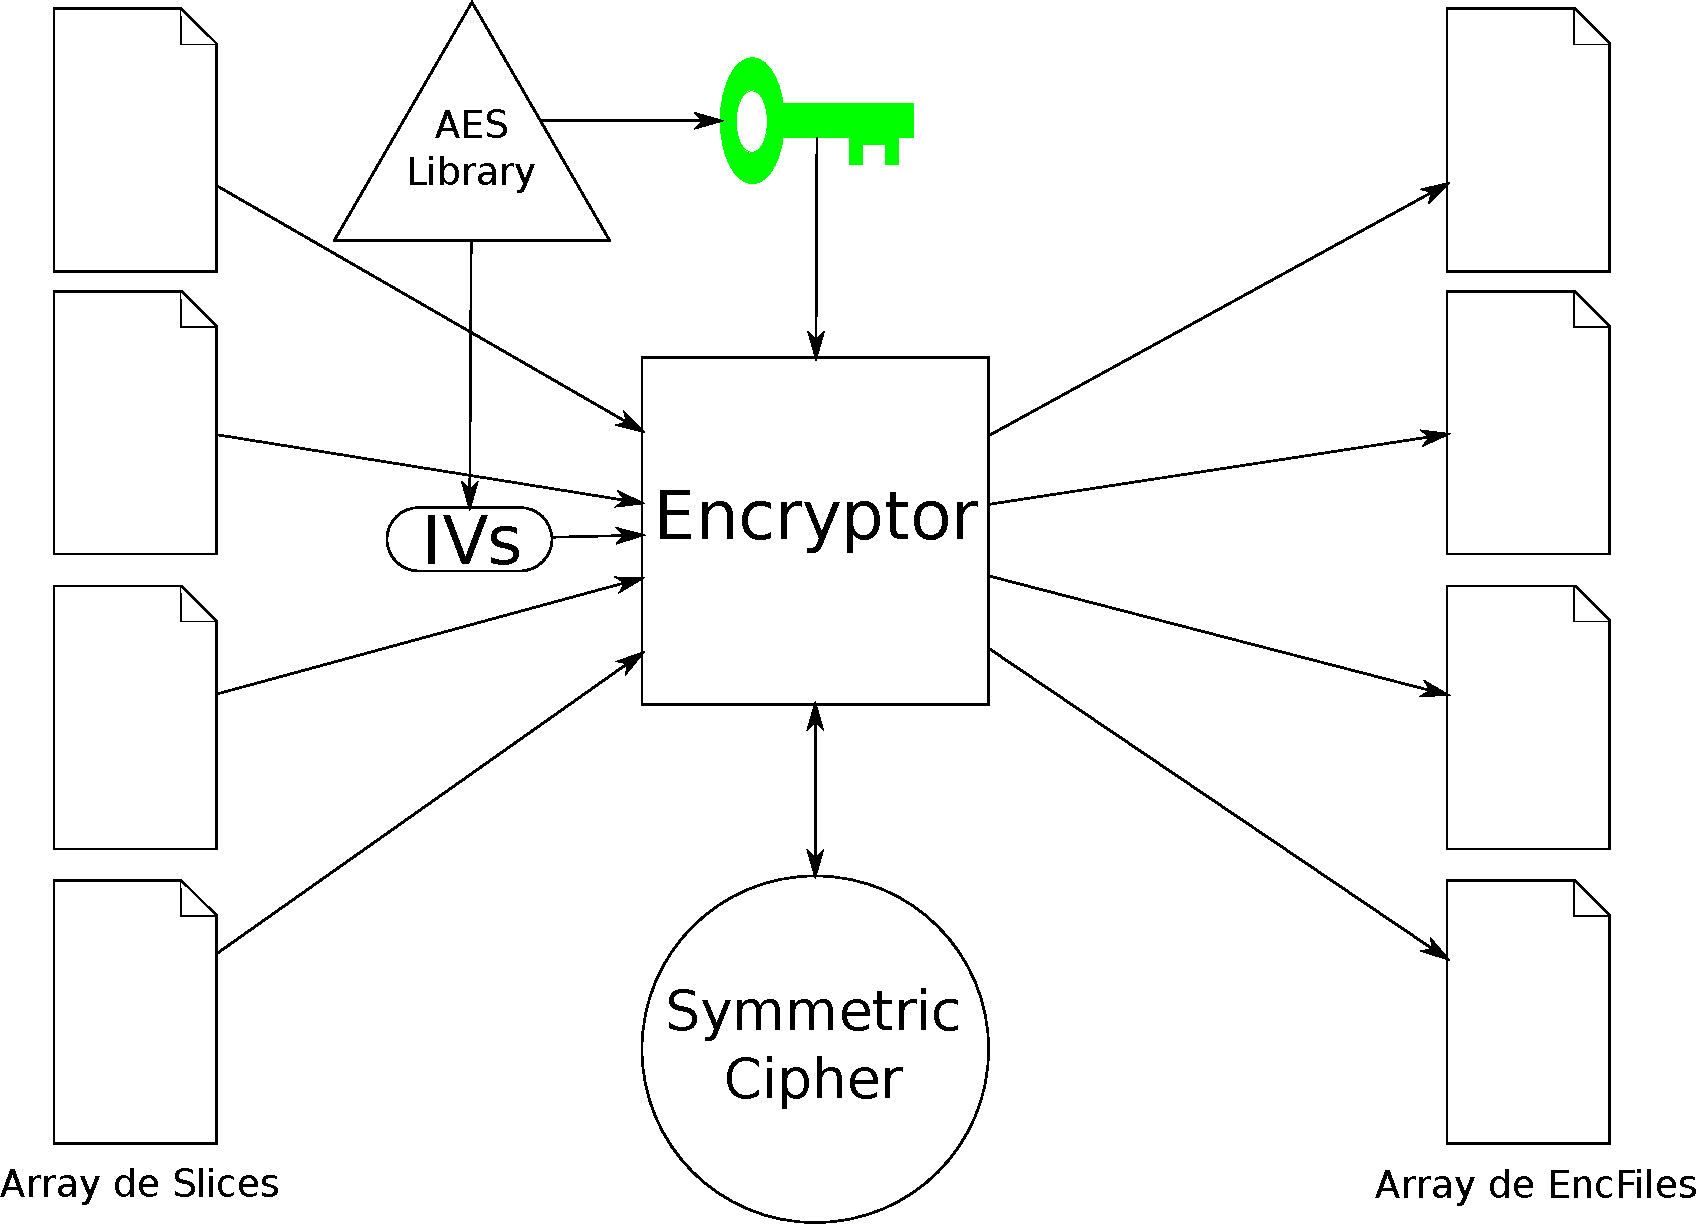
\includegraphics[scale=0.5]{Figures/Encryptor}
  \decoRule
  \caption[Encryptor]{Esquema general del funcionamiento del Encryptor}
  \label{fig:Encryptor}
\end{figure}

\begin{figure}[ht]
  \centering
  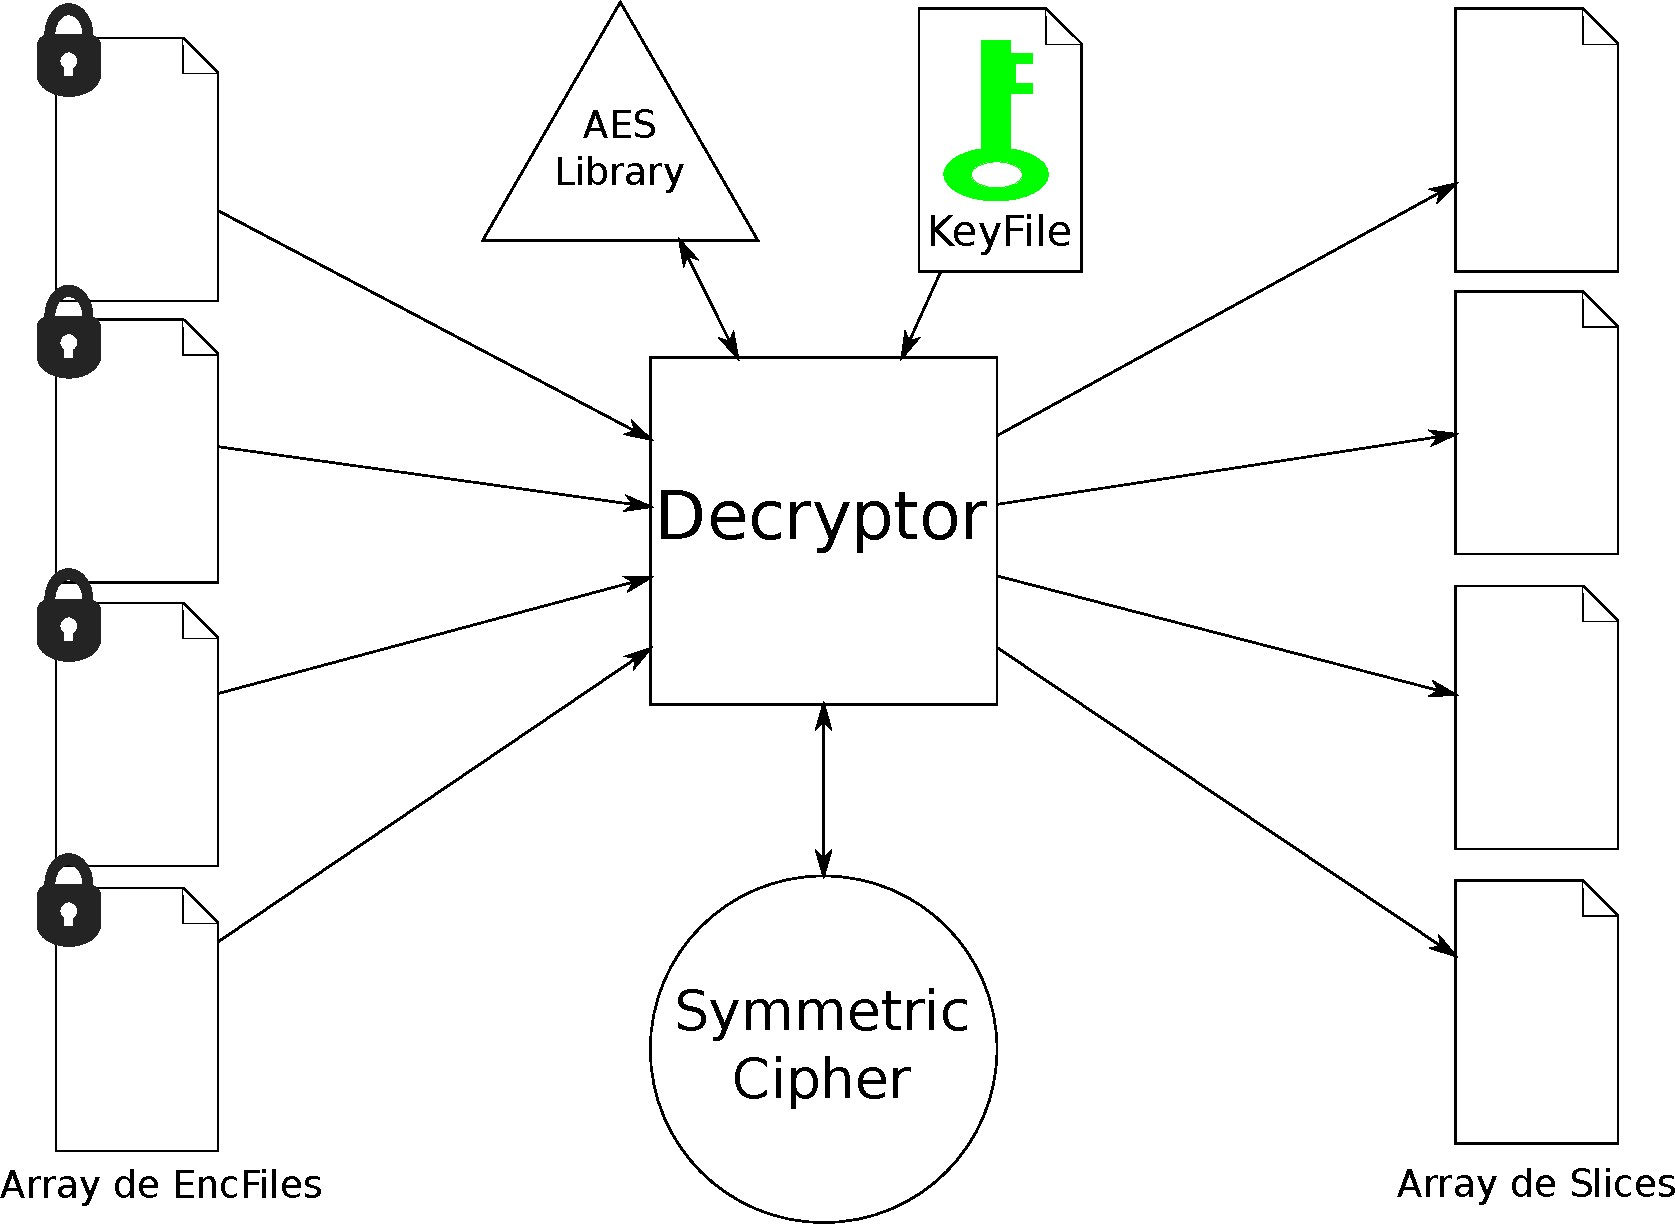
\includegraphics[scale=0.5]{Figures/Decryptor}
  \decoRule
  \caption[Decryptor]{Esquema general del funcionamiento del Decryptor}
  \label{fig:Decryptor}
\end{figure}

A pesar de que la seguridad que proporciona este prototipo no está completa (Ya
que es propenso a algunos ataques), sienta las bases de lo que será
la arquitectura de seguridad de la aplicación.

\subsection{Shatter 0.8}

A pesar de que ya teníamos confidencialidad en las Slices, había que
proporcionársela también al KeyFile. En este prototipo se crearon las siguientes
clases para lograrlo:

\begin{itemize}
  \item \keyword{EncKeyFile} -- En esta clase se almacena la clave simétrica
  cifrada usando para ello una clave asimétrica. Tiene una cabecera en la que
  se guardan algunos datos importantes.

  \item \keyword{EncKeyFileHeader} -- La cabecera del EncKeyFile. En ella se
  almacena una firma cifrada (HMAC) de la clave simétrica sin cifrar.

  \item \keyword{RSALibrary} -- Esta clase es la encargada de generar un par de
  claves asimétricas, de escribirlas y leerlas de un fichero y de cifrar
  un texto plano a uno cifrado, y viceversa.

  \item \keyword{Signature} -- Básicamente una clase para contener una firma.

  \item \keyword{SecureSignature} -- Contiene la firma comentada antes pero
  cifrada usando una clave asimétrica. Es una HMAC.

  \item \keyword{Signer} -- La clase que se encarga de recibir Slices, EncFiles,
  KeyFiles y demás y devolverlos firmados. Asimismo, se encarga de comprobar
  las firmas de todos estos ficheros para preservar la autenticidad de la
  información que portan. (Figura~\ref{fig:Signer})

  \item \keyword{RSAPSS} -- Esta clase incorpora todos los métodos necesarios
  para generar, a partir de un texto plano, un texto codificado y firmado
  usando el algoritmo RSASSA-PSS. También realiza el proceso inverso y puede
  verificar las firmas.
\end{itemize}

\begin{figure}[ht]
  \centering
  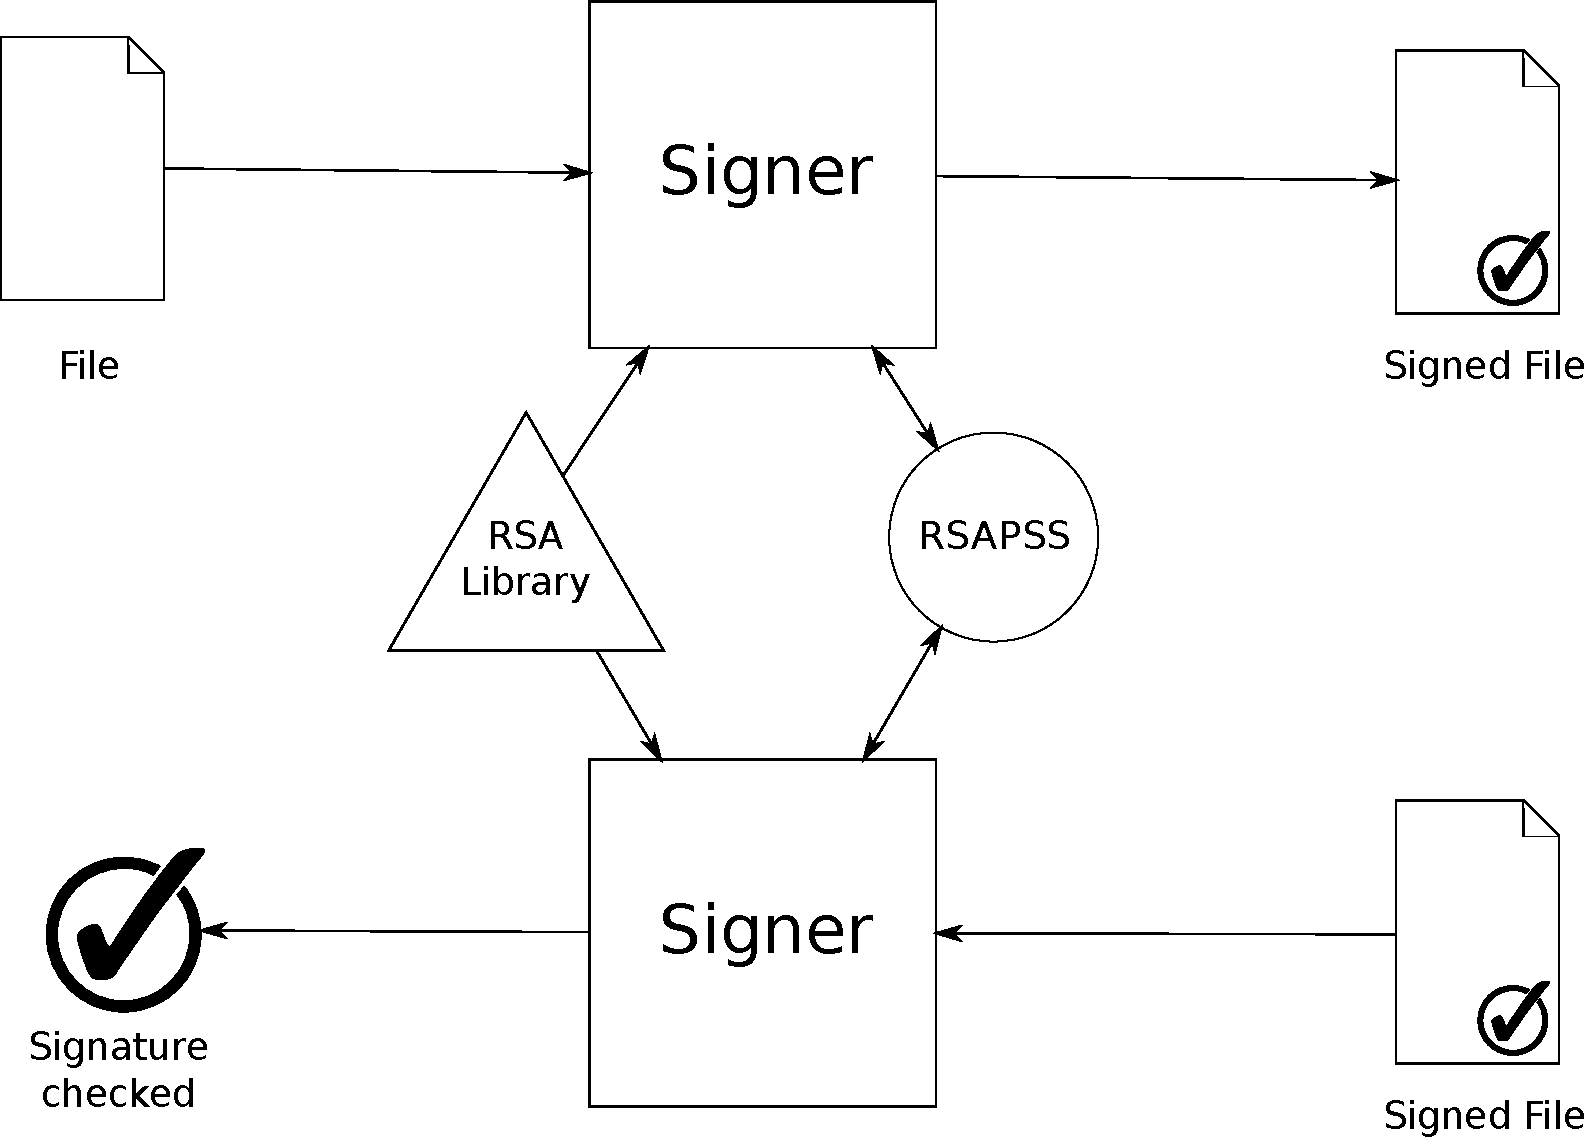
\includegraphics[scale=0.4]{Figures/Signer}
  \decoRule
  \caption[Signer]{Esquema general del funcionamiento del Signer}
  \label{fig:Signer}
\end{figure}

Con el prototipo anterior nos dimos cuenta de que, a parte de que teníamos que
generar un modo seguro de transmitir la clave simétrica, también teníamos que
proporcionar una manera de comprobar la autenticidad de los datos.

Debido a ello, incluimos una firma en el KeyFile y en las cabeceras de las
Slices y EncFiles (Figuras~\ref{fig:Slice_Header_2} y~\ref{fig:EncFile_Header_2}).
Nos dimos cuenta de que algunas firmas iban a ir en claro cuando viajasen de un
equipo a otro. Por ello se decidió la creación de una firma cifrada (HMAC),
para evitar posibles "mirones".

\begin{figure}[ht]
  \centering
  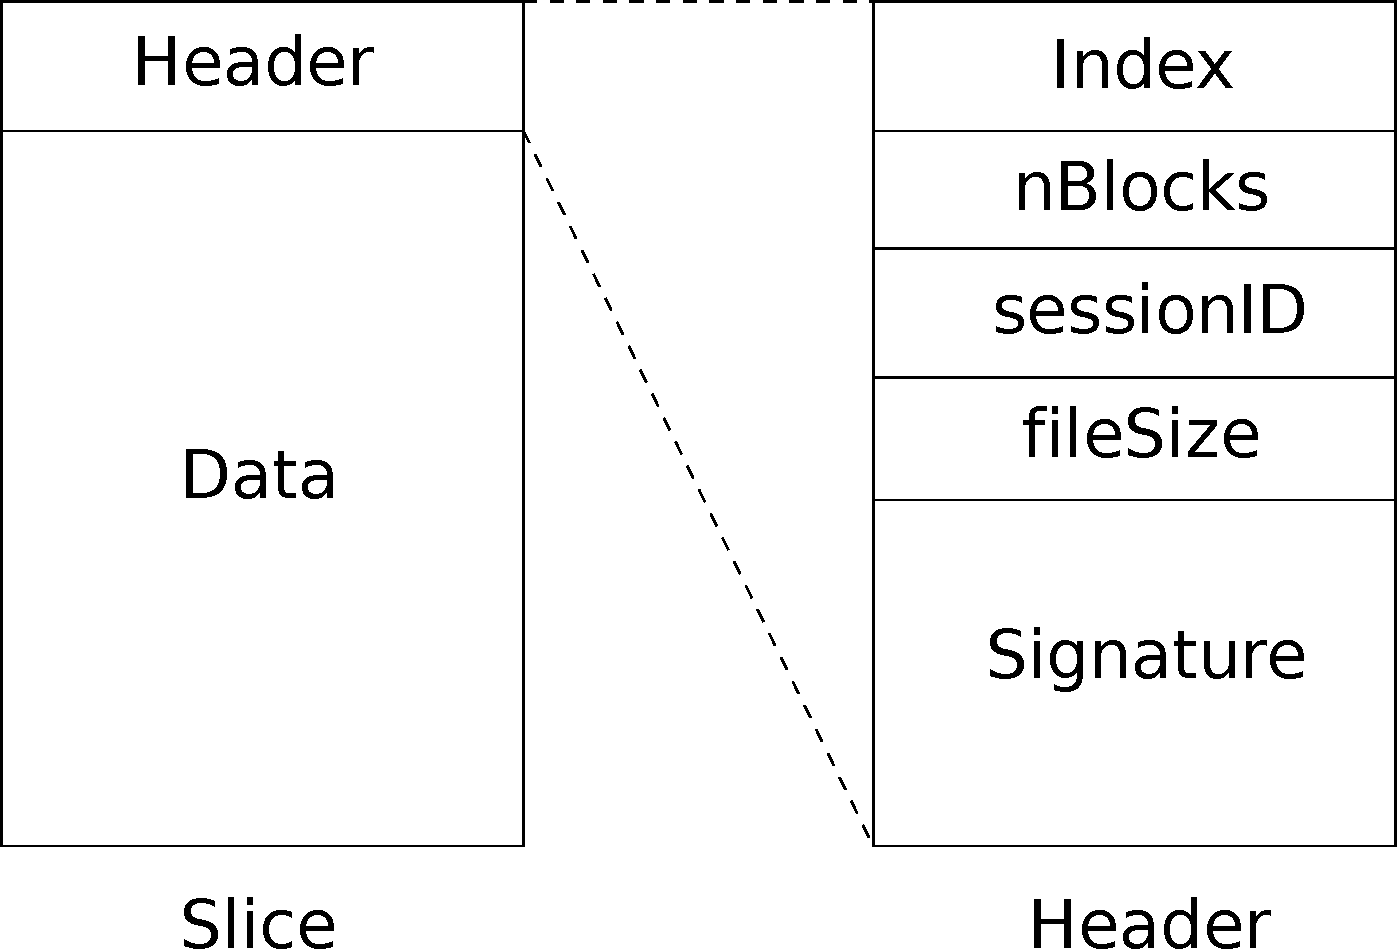
\includegraphics[scale=0.4]{Figures/Slice_Header_2}
  \decoRule
  \caption[Slice - Header (Versión final)]{Esquema general de las clases Slice y Header (Versión final)}
  \label{fig:Slice_Header_2}
\end{figure}

\begin{figure}[ht]
  \centering
  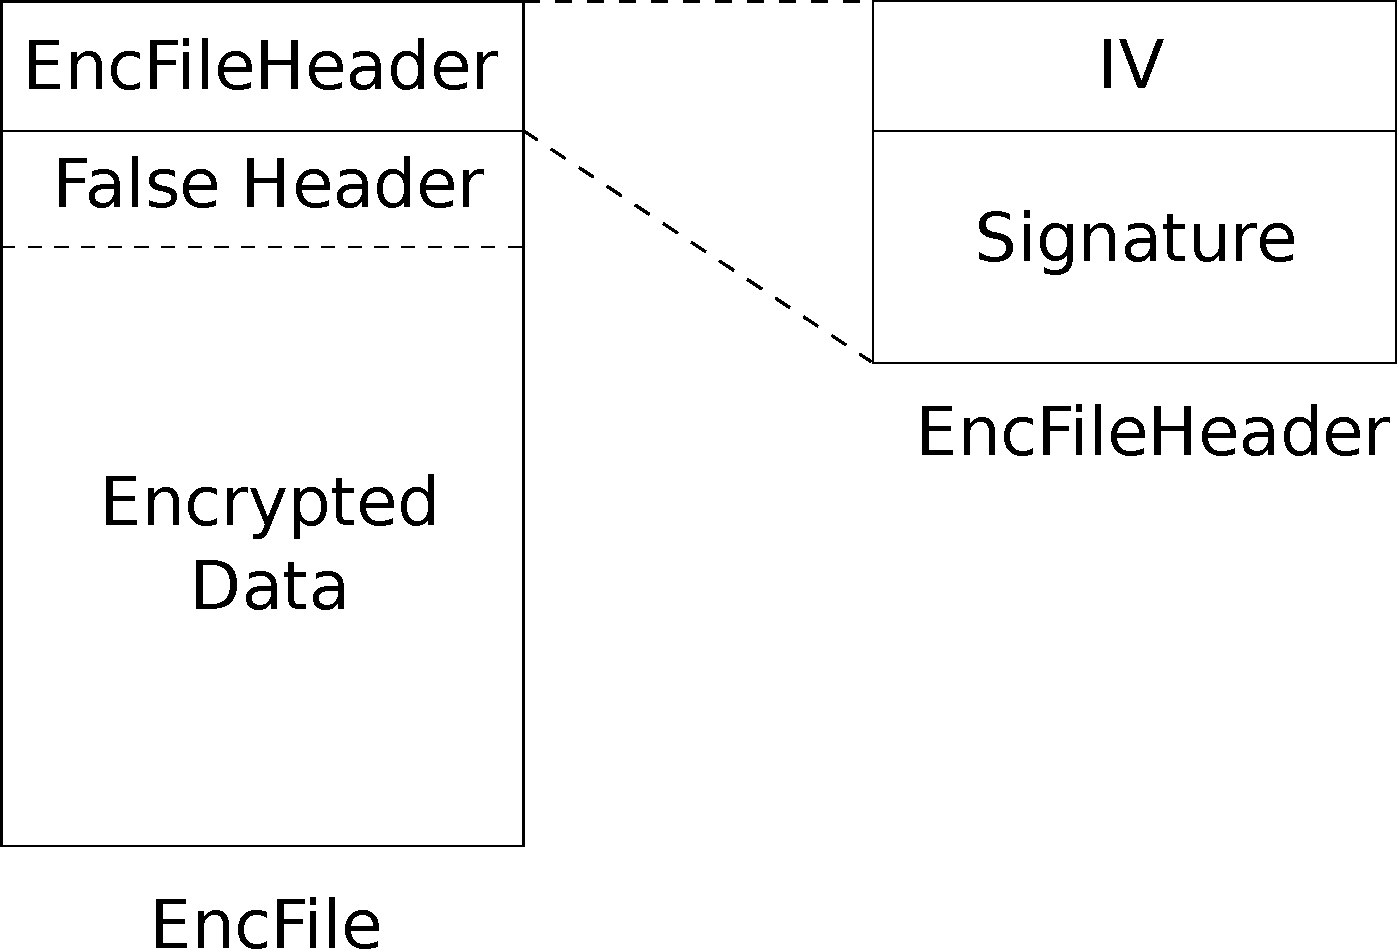
\includegraphics[scale=0.4]{Figures/EncFile_Header_2}
  \decoRule
  \caption[EncFile - EncFileHeader (Versión final)]{Esquema general de las clases EncFile y EncFileHeader (Versión final)}
  \label{fig:EncFile_Header_2}
\end{figure}

Además de las clases mencionadas anteriormente, también se desarrollaron otras
clases para generar Strings aleatorios, para leer y escribir los distintos
ficheros que intervienen en la aplicación, etc.

\subsection{Shatter 1.0}

Esta versión final de la aplicación está marcada por el salto a la plataforma
Android. Gran parte del código desarrollado en los anteriores prototipos se
siguió utilizando, sin embargo hubo que cambiar algunas clases:

\begin{itemize}
  \item \keyword{KeyStoreHandler} -- Esta clase se usa para realizar todas las
  operaciones necesarias con el KeyStore de Android. Se encarga de almacenar las
  claves, recuperarlas, usarlas para encriptar, firmar, etc.

  \item \keyword{HTTPClient} -- Un cliente HTTP muy sencillo que únicamente
  realiza peticiones GET.

  \item \keyword{ExternalStorage} -- Para interactuar con el External Storage de
  Android se creó una clase que incorpora algunos métodos para conseguir paths,
  descriptores de fichero o crear directorios.
\end{itemize}

A parte del desarrollo de estas clases, se trabajó también en un servidor HTTP
dedicado para almacenar los mensajes enviados por los distintos usuarios de la
aplicación.

Algunas clases, debido al cambio de plataforma, tuvieron que ser eliminadas.
El cambio más notorio fue la desaparición de las clases RSALibrary y RSAPSS,
ambas sustituidas por KeyStoreManager.

Un cambio menor fue la generación de un ID de sesión aleatorio para las
cabeceras de algunas clases (Anteriormente se usaba un resumen hash del
fichero).

El esquema general de la aplicación se puede dividir en dos: Una primera parte
se encarga de la división y cifrado del fichero (Figura~\ref{fig:abstractA}). La
otra se encarga de descargar del servidor los fragmentos cifrados y recomponer
el fichero original (Figura~\ref{fig:abstractB}).

\begin{figure}[ht]
  \centering
  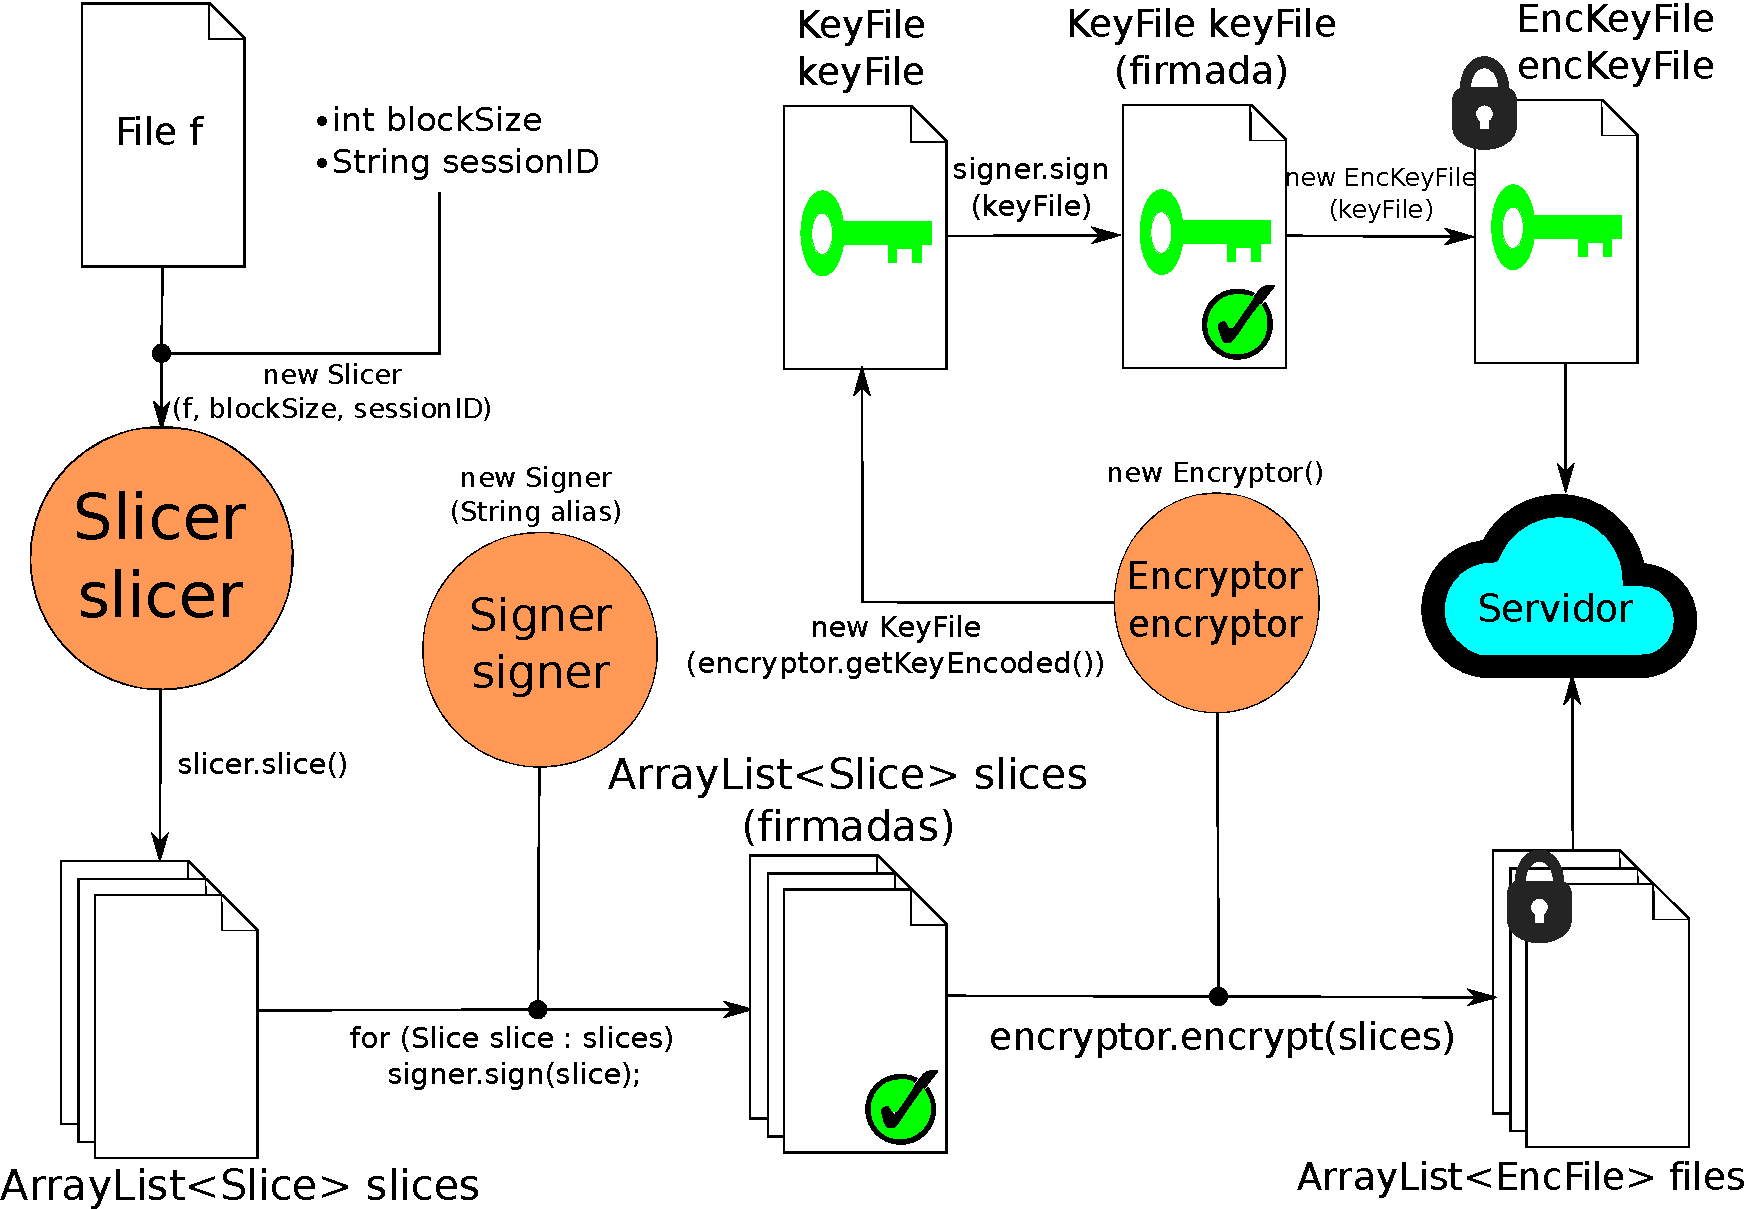
\includegraphics[scale=0.5]{Figures/abstractA}
  \decoRule
  \caption[Slice - Encrypt]{Esquema general de Slice - Encrypt, la primera parte en el proceso de comunicación de la aplicación}
  \label{fig:abstractA}
\end{figure}

\begin{figure}[ht]
  \centering
  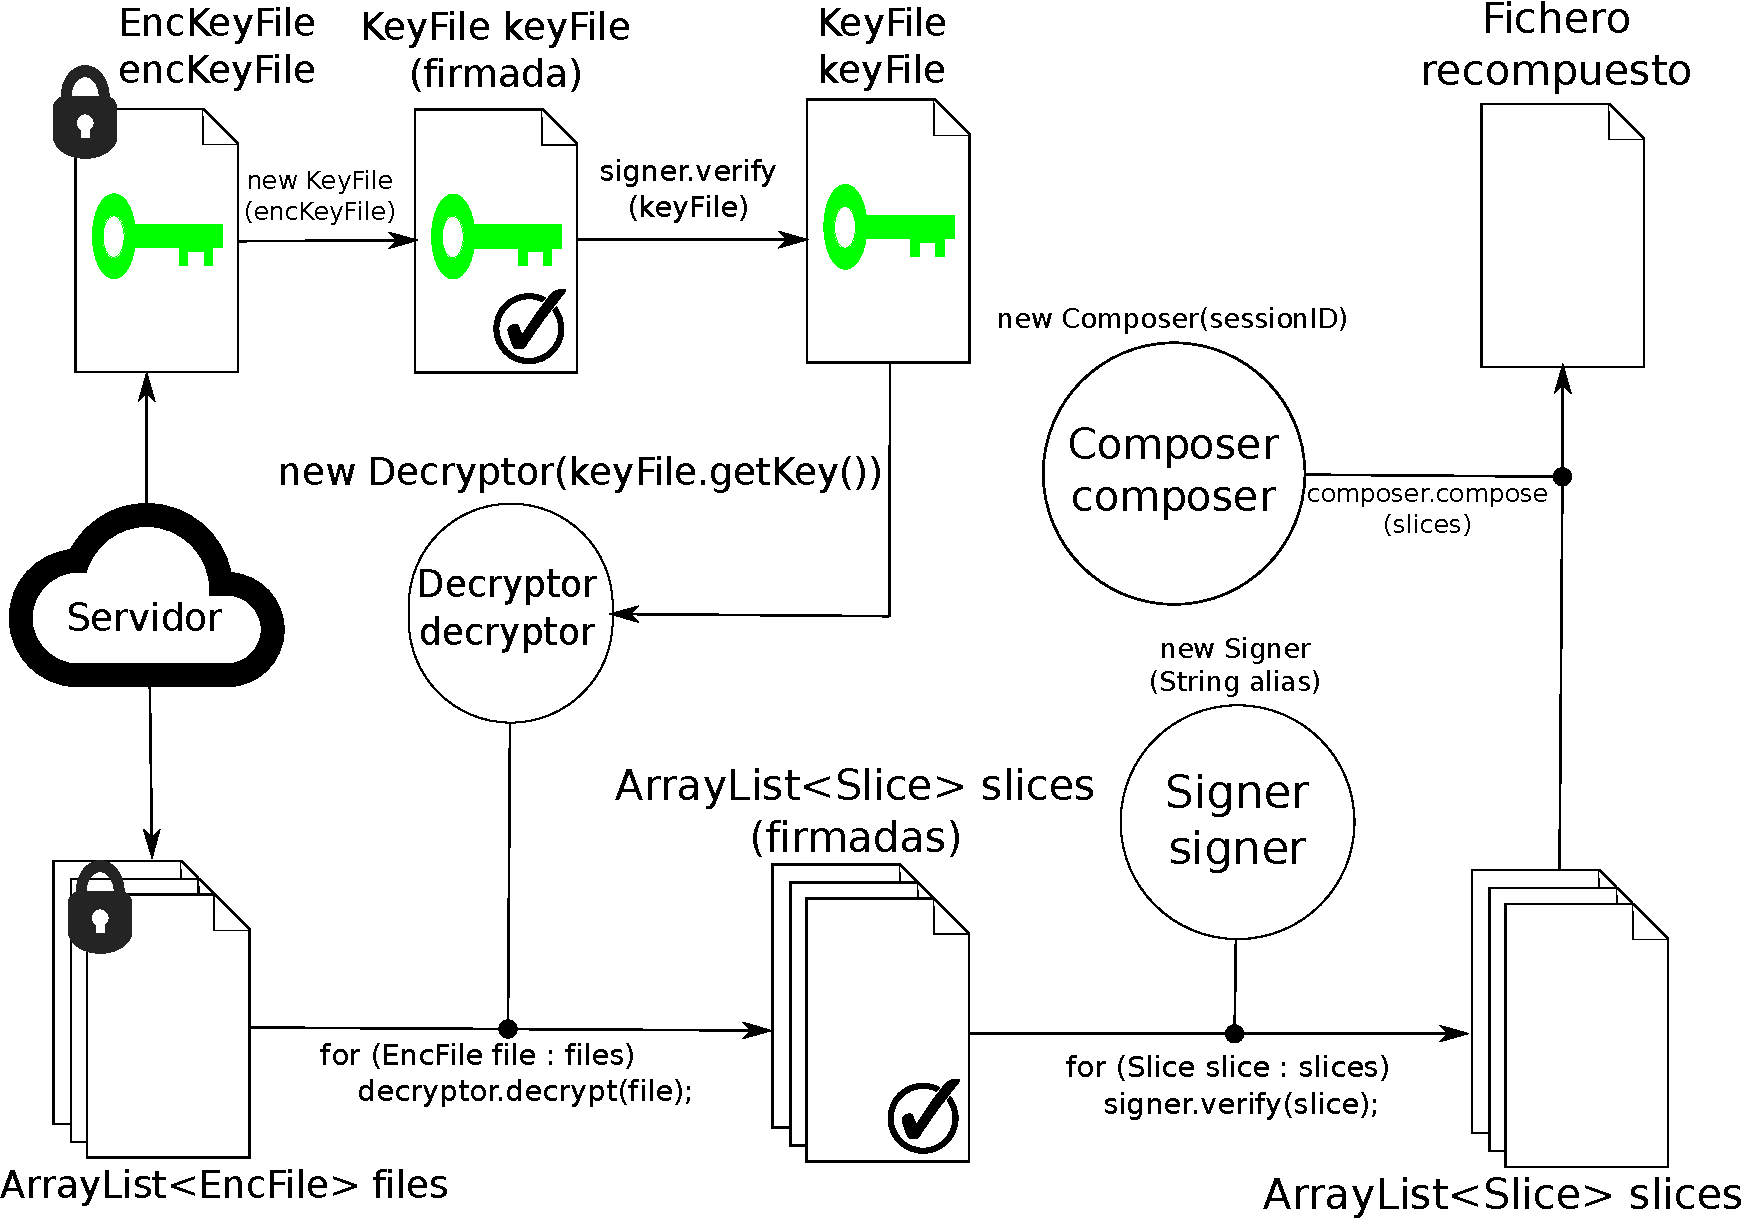
\includegraphics[scale=0.5]{Figures/abstractB}
  \decoRule
  \caption[Decrypt - Compose]{Esquema general de Decrypt - Compose, la parte final en el proceso de comunicación de la aplicación}
  \label{fig:abstractB}
\end{figure}
